% Rendu du sujet 4 (file M/M/1). Compiler avec : xelatex sujet4.tex (deux fois)
\documentclass[11pt,a4paper]{article}
\usepackage[a4paper,top=2.1cm,bottom=1.8cm,left=1.9cm,right=1.9cm,headsep=0.5cm]{geometry}
\usepackage[no-math]{fontspec}
\setmainfont{Inter}[Scale=0.88]
\setmonofont{DejaVu Sans Mono}[Scale=0.78]
\usepackage{polyglossia}\setmainlanguage{french}
\usepackage{amsmath,amssymb,icomma}
\usepackage{graphicx,xcolor,booktabs,tabularx,array,listings,fancyhdr,enumitem,tcolorbox,multicol}
\tcbuselibrary{raster}
\usepackage{lastpage,needspace}
\usepackage[hidelinks]{hyperref}

\definecolor{violet8}{HTML}{842577}
\definecolor{rouge8}{HTML}{E10717}
\definecolor{gris8}{HTML}{6B6B6B}
\definecolor{fond}{HTML}{F6F3F7}

\hypersetup{pdftitle={TP4 : Étude de la file d'attente M/M/1},
  pdfauthor={Esteban BERETTI--PRENANT},
  pdfsubject={Statistiques et Analyse de Données, Master Informatique I2A, Université Paris 8}}

\pagestyle{fancy}\fancyhf{}
\renewcommand{\headrulewidth}{0pt}
\fancyhead[L]{
\includegraphics[height=0.55cm]{paris8.png}}
\fancyhead[R]{\small\color{gris8}Statistiques et Analyse de Données · TP4}
\fancyfoot[C]{\small\color{gris8}\thepage\,/\,\pageref{LastPage}}
\fancypagestyle{premiere}{\fancyhf{}\renewcommand{\headrulewidth}{0pt}%
  \fancyfoot[C]{\small\color{gris8}\thepage\,/\,\pageref{LastPage}}}
\newcommand{\etiquette}[1]{\leavevmode{\scriptsize\addfontfeatures{LetterSpace=8}\color{gris8}\MakeUppercase{#1}}}

\newcommand{\question}[1]{\needspace{10\baselineskip}\vspace{0.5em}{\large\bfseries\color{violet8}#1}\par\vspace{0.25em}}
\newcommand{\lecture}{{\bfseries\color{rouge8}Lecture.}\ }
\newcommand{\resultat}{{\bfseries\color{violet8}Résultat.}\ }
% carte « chiffre clé » de la synthèse : couleur, chiffre, légende
\newcommand{\carte}[3]{\begin{tcolorbox}[colback=#1!7,colframe=#1!7,arc=3pt,boxrule=0pt,
  left=7pt,right=6pt,top=6pt,bottom=6pt]
  {\fontsize{19}{22}\selectfont\bfseries\color{#1}#2}\par\vspace{0.3em}{\footnotesize\raggedright #3\par}\end{tcolorbox}}

\lstset{basicstyle=\ttfamily,keywordstyle=\color{violet8}\bfseries,commentstyle=\color{gris8},
  language=Python,columns=fullflexible,keepspaces=true,frame=none,backgroundcolor=\color{fond},
  xleftmargin=4pt,framexleftmargin=4pt,aboveskip=4pt,belowskip=4pt,
  literate={é}{{\'e}}1{è}{{\`e}}1{à}{{\`a}}1{ê}{{\^e}}1{É}{{\'E}}1{λ}{{$\lambda$}}1{μ}{{$\mu$}}1
    {ρ}{{$\rho$}}1{≤}{{$\le$}}1{≥}{{$\ge$}}1{·}{{$\cdot$}}1}

\tcbset{coquille/.style={colback=rouge8!5,colframe=rouge8!70,boxrule=0.5pt,arc=2pt,
  left=5pt,right=5pt,top=3pt,bottom=3pt,fontupper=\small}}

\setlength{\parindent}{0pt}\setlength{\parskip}{0.35em}
\setlist{nosep,leftmargin=1.2em}

\begin{document}

% ---------- En-tête de la première page ----------
\thispagestyle{premiere}
\vspace*{-1.2cm}
\noindent\begin{minipage}[c]{0.5\linewidth}
\includegraphics[height=1.55cm]{paris8.png}\end{minipage}%
\begin{minipage}[c]{0.5\linewidth}\raggedleft\small\color{gris8}
Master Informatique I2A\\Année 2026-2027\end{minipage}

\vspace{0.5cm}
{\footnotesize\bfseries\addfontfeatures{LetterSpace=14}\color{rouge8}STATISTIQUES ET ANALYSE DE DONNÉES · RENDU}\par
\vspace{0.5em}
{\fontsize{24}{29}\selectfont\bfseries TP4 : Étude de la file d'attente M/M/1\par}
\vspace{0.5em}
{\large\color{violet8}Partie A : la loi exponentielle et l'absence de mémoire\par}
\vspace{0.6em}
{\color{violet8}\rule{0.32\linewidth}{2pt}}{\color{rouge8}\rule{0.18\linewidth}{2pt}}\par
\vspace{0.7em}

\begin{tcolorbox}[colback=fond,colframe=fond,arc=3pt,boxrule=0pt,left=10pt,right=10pt,top=5pt,bottom=5pt]
\renewcommand{\arraystretch}{1.35}
\begin{tabularx}{\linewidth}{@{}p{2.2cm} >{\raggedright\arraybackslash}X p{2.2cm} >{\raggedright\arraybackslash}p{3.2cm}@{}}
\etiquette{Auteur} & \textbf{Esteban BERETTI--PRENANT} & \etiquette{Enseignant} & M. Zerzeri \\
\etiquette{Formation} & Master Informatique I2A, Université Paris 8 & \etiquette{Date} & 25/11/2026 \\
\etiquette{Outils} & Python (numpy, matplotlib) & & \\
\etiquette{Dépôt} & \multicolumn{3}{l}{\href{https://github.com/Este34/presentation_statistique}{\color{violet8}github.com/Este34/presentation\_statistique}\ \ {\color{gris8}\small(code, tests, notebooks)}} \\
\end{tabularx}
\end{tcolorbox}

% ---------- Synthèse ----------
\vspace{0.3em}{\large\bfseries\color{violet8}Synthèse}\par\vspace{0.1em}
Dans la file M/M/1, les temps de service suivent une loi exponentielle. Ce rendu étudie cette loi
(partie A du sujet) : ses deux paramètres de forme, et la propriété qui la caractérise, l'absence
de mémoire.

{\small
\renewcommand{\arraystretch}{1.25}
\begin{tabularx}{\linewidth}{@{}>{\leavevmode\color{violet8}\bfseries}p{1.0cm} >{\raggedright\arraybackslash}X >{\raggedright\arraybackslash}p{5.2cm}@{}}
\toprule
 & \textbf{Résultat} & \textbf{Pourquoi} \\ \midrule
A.1 & $E[X] = \sigma_X = \dfrac{1}{\lambda}$ : moyenne et écart-type égaux & intégration par parties \\
A.2 & $P(X \ge x + t \mid X \ge x) = P(X \ge t)$ : ce qui reste à attendre ne dépend pas de ce qui est écoulé & $\{X \ge x + t\} \subset \{X \ge x\}$ et $e^{-\lambda(x+t)}/e^{-\lambda x} = e^{-\lambda t}$ \\
A.3 & c'est la \textbf{seule} loi sans mémoire & $G(x+t) = G(x)G(t)$ force $G(x) = e^{-\lambda x}$ \\
\bottomrule
\end{tabularx}}

\question{A.1 · Moyenne et écart-type}
\resultat La densité est $f(x) = \lambda e^{-\lambda x}$ pour $x \ge 0$ (dérivée de
$1 - P(X \ge x) = 1 - e^{-\lambda x}$). Par intégration par parties,
$E[X] = \big[-x e^{-\lambda x}\big]_0^{\infty} + \int_0^{\infty} e^{-\lambda x}\,dx = \frac{1}{\lambda}$,
puis $E[X^2] = \frac{2}{\lambda}E[X] = \frac{2}{\lambda^2}$, donc
$\operatorname{Var}X = E[X^2] - E[X]^2 = \frac{1}{\lambda^2}$ et $\boxed{E[X] = \sigma_X = 1/\lambda}$.

\question{A.2 · L'absence de mémoire}
\resultat Pour $x, t \ge 0$, l'événement $\{X \ge x + t\}$ est inclus dans $\{X \ge x\}$, donc
$P(X \ge x + t \mid X \ge x) = \frac{P(X \ge x+t)}{P(X \ge x)} = \frac{e^{-\lambda(x+t)}}{e^{-\lambda x}} = e^{-\lambda t} = P(X \ge t)$.
Si $X$ est une durée de vie, la durée de vie restante ne dépend pas de l'âge.

\vspace{0.5em}{\large\bfseries\color{violet8}A.3 · La seule loi sans mémoire}\par\vspace{0.25em}
\resultat Avec $G(x) = P(X \ge x) > 0$, la propriété s'écrit $G(x + t) = G(x)\,G(t)$ pour tous
$x, t \ge 0$. Alors $\ln G$ est additive et décroissante : elle est linéaire sur les rationnels, puis
sur tous les réels grâce à la monotonie. Donc $G(x) = e^{-\lambda x}$ avec $\lambda > 0$ : $X$ suit
une loi exponentielle.

\begin{center}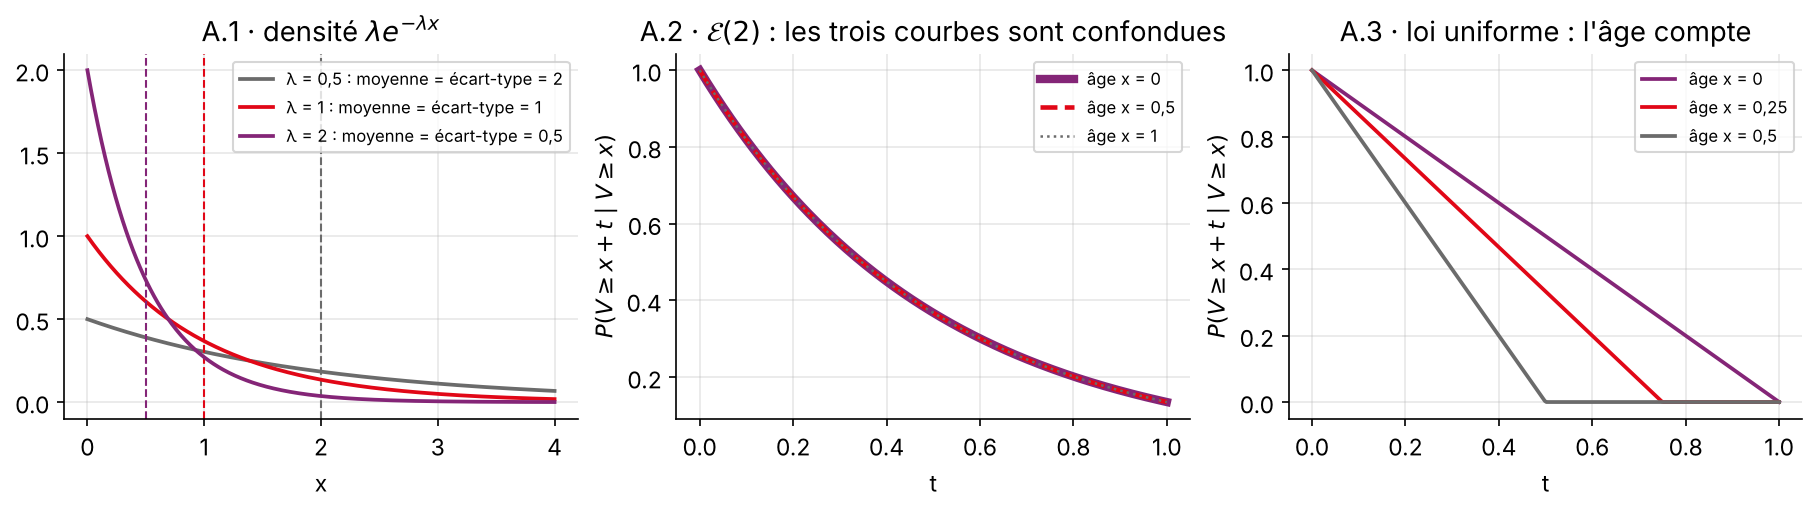
\includegraphics[width=\linewidth]{../../sujets/sujet4/figures/s4a_theorie.png}\end{center}
\vspace{-0.6em}
\lecture À gauche, plus $\lambda$ est grand, plus les durées sont courtes ; la moyenne $1/\lambda$
(tirets) est aussi l'écart-type. Au centre, pour $\mathcal E(2)$, la probabilité de durer encore
$t = 0{,}5$ vaut $e^{-1} = 0{,}368$ quel que soit l'âge : les trois courbes sont confondues. À droite,
contre-exemple : pour la loi uniforme sur $[0, 1]$, la probabilité de durer encore $0{,}25$ passe de
$0{,}75$ (âge 0) à $0{,}5$ (âge $0{,}5$) : plus elle a duré, plus la fin est proche.

\vspace{0.4em}
\textbf{\color{violet8}Conclusion.} La loi exponentielle a une moyenne et un écart-type égaux à
$1/\lambda$, et c'est la seule loi sans mémoire. Pour la file M/M/1, cela veut dire qu'un client en
cours de service a toujours un temps restant de même loi, quel que soit le temps déjà passé.
\label{fin}
\end{document}
